\section{Analyse des données}

\begin{frame}
  \frtt{Analyse des données}
Données: \\
	\begin{itemize}
		\item VLBI Earth Orientation Solution OPA2015a	
		\item Rigid Earth Nutation (Souchay et al. 1997)
	\end{itemize}
	\vspace{0.5cm}
	L'équation des moindres carrés: \\
	$X(t) + i \times Y(t) = \sum\limits_{j=1}^{40} (\widetilde{A}_{j} \times e^{(\omega_{j}*t + \varphi_{j})})$ \\
	$\widetilde{A} = A_{Re} + i \times A_{Im}$ \\

	\vspace{0.5cm}
	$\widetilde{A}$ : amplitude \\
	$\omega$ : fréquence \\
	$\varphi$ : phase \\
	$t$ : temps
\end{frame}

\begin{frame}
  \frtt{Amplitude Ajustées}
	\begin{center}
		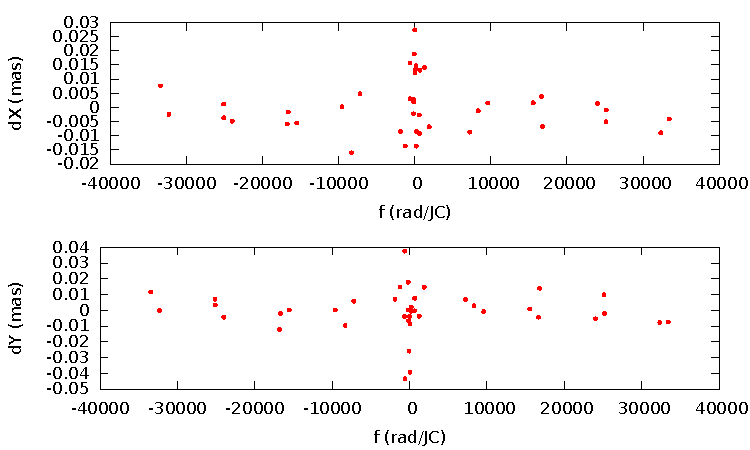
\includegraphics[width=1.0\textwidth]{amplitude_freq.pdf}
	\end{center}
\end{frame}

\begin{frame}
  \frtt{Corrélation}
  \centerline{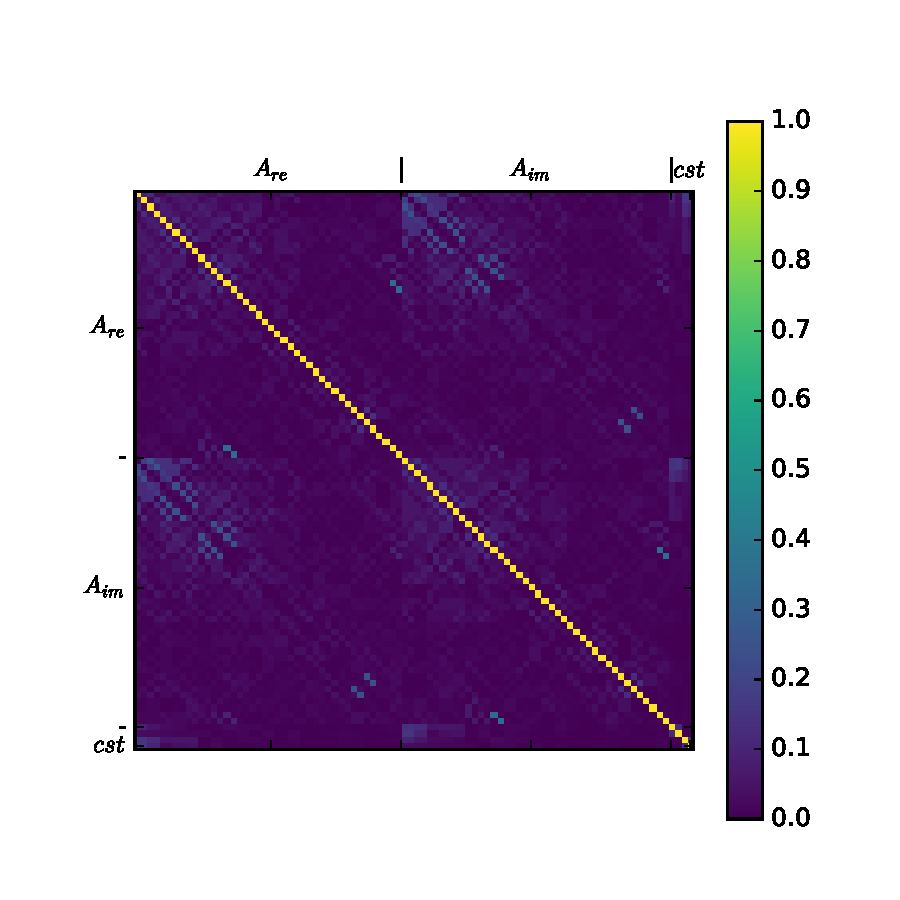
\includegraphics[width=0.8\textwidth]{fit_amplitude_correlation.pdf}}
\end{frame}


\begin{frame}
  \frtt{Comparaison entre série ajusté et observation}
	\begin{center}
		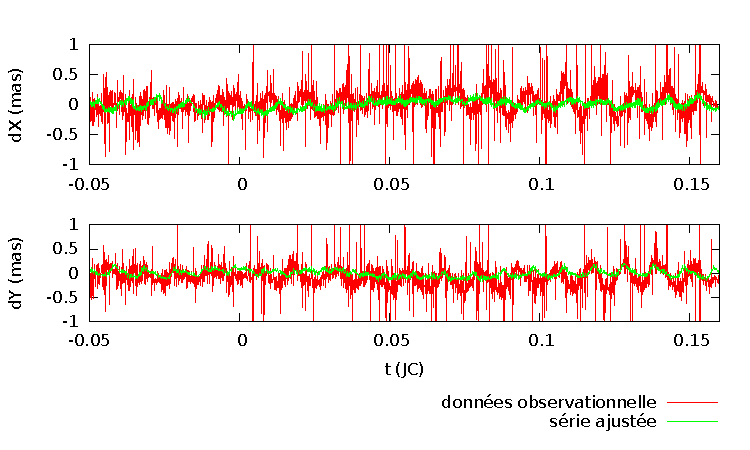
\includegraphics[width=1.0\textwidth]{fit_amplitude_ser_obs.pdf}
	\end{center} 
\end{frame}

